\documentclass[
  a4paper,
  emulatestandardclasses,
  abstract,
  parskip
]{scrreprt}

\usepackage[T1]{fontenc}
\usepackage[english]{babel}

\usepackage{bm}
\usepackage{a4wide}
\usepackage{siunitx}
\usepackage{authblk}
\usepackage{physics}
\usepackage{amsthm}
\usepackage{amsmath}
\usepackage{amssymb}
\usepackage{csquotes}
\usepackage{biblatex}
\usepackage{enumerate}
\usepackage{hyperref}
\usepackage{graphicx}

\newcommand{\builddir}[1]{build/#1}
\newcommand{\imagedir}[1]{images/#1}

\addbibresource{literature.bib}

\numberwithin{equation}{section}

\subject{Many Body Quantum Optics}
\title{High-precision time-averaged optical potentials for ultracold atoms
  \vskip 1em
  \includegraphics[width=9cm]{\builddir{emblem.pdf}}
}
\subtitle{Bachelor thesis by}
\author[1]{Bodo Kaiser}
\affil[1]{Ludwig-Maximilians-Universität München}
\affil[ ]{\textit{bodo.kaiser@physik.uni-muenchen.de}}
\publishers{Supervision by Prof. Dr. Immanuel Block, Dr. Monika Aidelsburger
  and Christian Schweitzer.}

\begin{document}

\maketitle
\cleardoublepage

\begin{abstract}
Ultracold atoms in optical lattices open up a wide range of possibilities
to simulate many-body quantum phenomena, which would elsewise be neither
computationally nor experimentally tangible.

The topology of the optical lattice is a decisive property of these kind
of experiments and therefore of major interest. Recently, efforts have been
reported to create novel optical potentials through the use of digital
micromirror arrays that permit alterations of localized potentials. Though
promising results have been achieved --- in particular for static potentials
--- limitations due to the mechanical nature of these mirror arrays arise,
for instance, with regard to dynamical control.

In the present work we present an alternative implementation of localized
optical lattice potentials based on acousto-optic deflectors and
direct digital synthesizers.

We will give a brief theoretical introduction into the main concepts, i.e.\
the interaction of neutral atoms with optical potentials as well as the
general operation of direct digital synthesizer and acousto-optic deflectors.
From the physics we can derive the requirements imposed on the technical
implementation of the \gls{rf} signal source and the deflection.

We will find that even though the platform of digital signal synthesis
generally suites our application in terms of modulation capabilities and
resolution, the particular implementation of the \gls{ad9910} demonstrates
several shortcomings.

In the second part we characterize the deflection efficiency of the
acousto-optic deflectors. Towards the end we try to minimize the variance of
the deflection efficiency by performing a random search on the amplitude
segments of the \gls{rf} signal. It turns out that the deflection efficiency
is a highly non-linear function of the applied \gls{rf} power and frequency.
Furthermore minimization of the deflection efficiency variances proves to be
very unstable. Though we can largely preclude electronic defects to be the
source of this behaviour, further investigation is required.
\end{abstract}


\tableofcontents

\chapter{Introduction}

Many quantum systems studied in condensed matter physics are experimentally
challenging to access as any interactions can destroy the carefully prepared
quantum states. As way forward, experiments with ultracold atoms in
optical lattices give us a highly contorllable environment, giving us the
opportunity to simulate and explore quantum effects and expand our current
understanding of quantum mechanics and statistical physics \cite{Gross2017}.

The central idea behind these types of experiments is to cool down neutral
atoms to micro Kelvin and below, and load them into an optical lattice. At
these temperatures atoms demonstrate quantum behaviour. The optical lattices
act as periodic potentials analogue to the periodic potential found inside
solid state crystal lattices \cite{Lewenstein2007}. Unlike to i.e. real solids
where we have limited prospects to amend a systems properties, lasers driven
by state of the art optics and electronics give us a wide range of well
controllable parameters.

\begin{figure}[h]
  \centering
  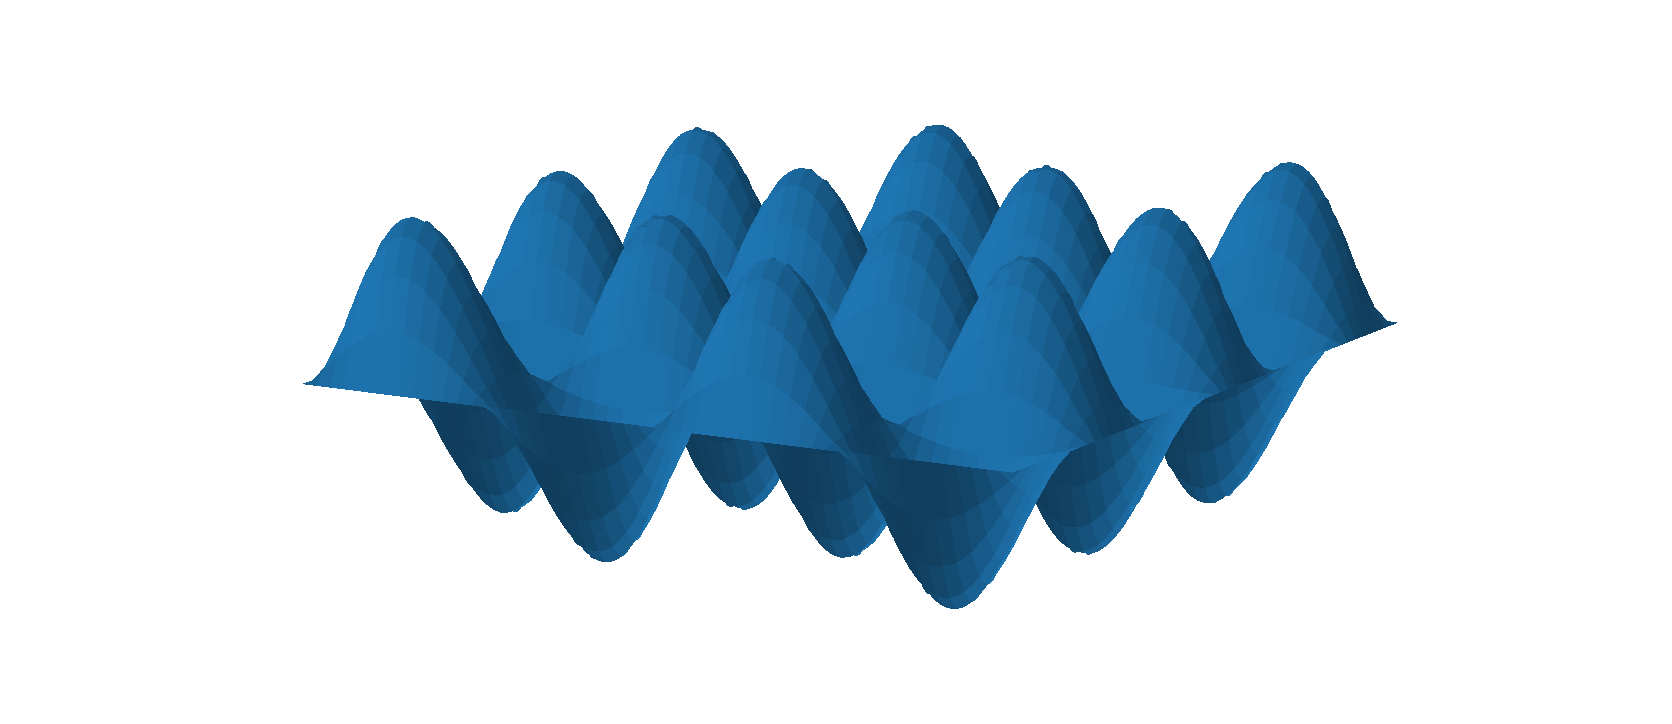
\includegraphics[width=.8\textwidth]{images/optlat/default.pdf}
  \captionsetup{width=.8\textwidth}
  \caption{Periodic potential of a 2D optical lattice. If the kinetic energy
  of the atoms is below the potential energy of the lattice, the atoms will
  locate around the potential minimas.}
  \label{fig:optlat}
\end{figure}

One of the parameters of interest is the ability to apply local potentials
to the system, that can be used to, among others, study lattice inpurities
or quantum interactions. In this work we will present and characterize one
possible implementation of such a local potential generating apparatus.

\section{Related Work}

Local manipulations of atoms inside optical lattices have been known for some
time in the embodiment of optical tweezers that allow trapping, stacking and
sorting of particles \cite{Tadmor2004}. Yet, only recently attempts to
interact with local particle clusters through high-precision time-averaged
optical potentials have been reported \cite{Roy2016}.

In the following we continue on the laid out work \cite{Hertlein2017} which
provided us with an optical setup for single-site manipulation using
\gls{aod} as well as considerations with regard to aperture limited
gaussian beam propagation.

\chapter{Experimental Setup}

For the experimental setup we adopted the setup described in \cite{Hertlein2017}.



\printbibliography

\end{document}
